\chapter{Porównanie wydajności baz relacyjnych i nierelacyjnych}

W poprzednich rozdziałach skupiliśmy się na porównaniu czysto teoretycznym oraz praktycznym. W tym rozdziale poruszymy rzeczywiste różnice po zaimplementowaniu dwóch rozwiązań w jednym projekcie. Obie bazy danych są postawione na zewnętrznym serwerze, opóźnienia połączenia w obu przypadkach są porównywalne, więc skupmy się na czasie odpytywania.

\section{Wnioski z analizy czasu wyszukiwania między bazami}
Przy blisko pięćdziesięciu próbach wykres prezentuje się następująco:
\begin{figure}[h]
    \centering
    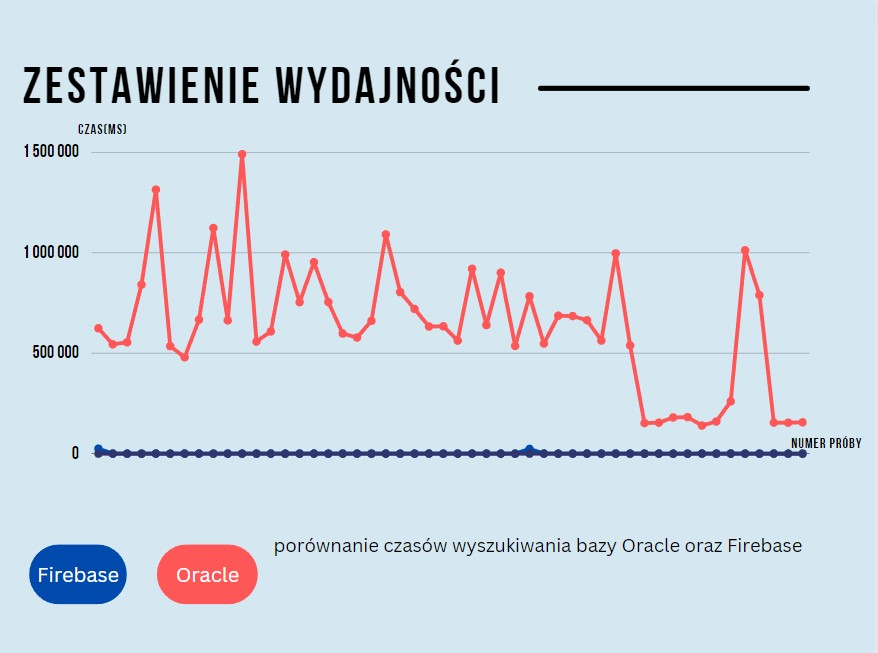
\includegraphics[width=0.8\linewidth]{./img/wykres.jpg}
    \caption{Wykres przedstawiający czas zapytania w milisekundach dla każdej próby}
    \label{fig:Wykres}
\end{figure}

\subsection{Analiza czasu reakcji i skuteczności cache}
Dane do powyższego wykresu, zostały pobrane z tabeli \textit{SEARCHING} opisanej w poprzednim rozdziale. Na osi Y widzimy czas w milisekundach potrzebny do pobrania wszystkich rekordów z bazy danych oraz przefiltrowania ich wobec preferencji użytkownika i zwróceniu do wyświetlenia użytkownikowi. Jak widzimy na powyższym wykresie różnica w wydajności działania bazy danych Firebase nad bazą danych Oracle jest miażdżąca. Z tej różnicy możemy wyciągnąć wniosek, iż Firebase jest wydajniejszy i bardziej przyszłościowy w stosunku do bazy relacyjnej Oracle.

Bazy nierelacyjne cechują się ogromną wydajnością i prędkością przeszukiwania, nie występuje tam tabelaryzacja jak po stronie baz relacyjnych, co ułatwia strukturę. Dla programistów implementacja jest dużo prostsza, bo wymaga tylko jednego serwisu do dodawania, usuwania oraz przeszukiwania rekordów, natomiast dla bazy relacyjnej potrzebujemy budować konkretne zapytania, jeśli mamy więcej warunków do wyszukiwania. Na przykładzie aplikacji \textit{FindYourGame} stworzonej w celu porównania baz relacyjnych i nierelacyjnych na przykładzie Firebase oraz Oracle database, dochodzimy do wniosku iż baza danych Firebase jest około 10000 razy wydajniejsza.

Chociaż wyniki wykresu sugerują, że Firebase jest znacząco szybszy niż Oracle, ważne jest również, aby zanalizować sposób, w jaki obie bazy danych radzą sobie z cache'owaniem danych. W przypadku Firebase, mechanizmy cache'owania są wbudowane i automatycznie synchronizują dane na urządzeniach klienckich. W przypadku Oracle, mechanizmy te są zazwyczaj bardziej konfigurowalne i mogą wymagać zastosowania dodatkowych narzędzi, takich jak Oracle Coherence.

\subsection{Skalowalność i zasoby}
Wydajność nie jest jedyną metryką, którą należy uwzględnić przy wyborze bazy danych. Skalowalność, zarówno wertykalna, jak i horyzontalna, jest równie krytyczna. Firebase, będący bazą nierelacyjną, oferuje znaczące korzyści w zakresie skalowalności horyzontalnej, dzięki czemu łatwo można go rozszerzyć dodając więcej maszyn. Oracle, choć skalowalny wertykalnie, może wymagać znaczących inwestycji w sprzęt i licencje przy dużej ilości danych.

\subsection{Koszty}
Firebase, oferowany jako usługa w chmurze, ma model cenowy zorientowany na zużycie, co może być korzystne dla start-upów i małych firm. Oracle, z drugiej strony, może wymagać znacznych inwestycji początkowych, zwłaszcza gdy licencje i koszty sprzętu są uwzględnione w równaniu.

\subsection{Kompleksowość zapytań}
Jednym z ograniczeń baz nierelacyjnych jest brak wsparcia dla złożonych zapytań i operacji, takich jak złączenia JOIN, które są standardem w bazach relacyjnych. W przypadku aplikacji wymagających złożonych zapytań i analiz, Oracle może oferować znacznie większą elastyczność.

\subsection{Bezpieczeństwo i zarządzanie danymi}
Oracle, będący jednym z najstarszych graczy w branży, oferuje znacznie bardziej rozbudowane opcje zarządzania i bezpieczeństwa danych. Firebase, choć łatwy w użyciu, może nie oferować tak zaawansowanych mechanizmów zarządzania danymi, co może być krytyczne dla przedsiębiorstw o dużej skali i regulowanych sektorach.

\section{Podsumowanie}
Mimo że nasze badania wskazują na znaczącą przewagę Firebase w kontekście wydajności odpytywania, wybór między Firebase a Oracle jako bazą danych nie powinien opierać się wyłącznie na tej jednej metryce. Wybór odpowiedniej bazy danych powinien również uwzględniać czynniki takie jak skalowalność, koszty, możliwości zapytań, bezpieczeństwo i zarządzanie danymi. W zależności od specyficznych potrzeb i wymagań projektu, każda z tych baz danych może okazać się bardziej odpowiednia.
